\documentclass{article}
\usepackage{ctex}
\usepackage{graphicx}
\usepackage{geometry}
\usepackage{amsmath}
\usepackage{booktabs}
\usepackage{pgfplots}
\pgfplotsset{compat=1.17}

\geometry{a4paper, margin=2.5cm}

\begin{document}

% ====================== 抄袭警示声明 ======================
\begin{center}
\vspace*{2cm}
\Large\textbf{\color{red}⚠️ 重要声明}

\vspace{0.8cm}
\large
本文档仅作为学习思路、仿真原理参考资料。\\
严禁直接复制全文提交作为个人实验报告，抄袭会造成课程成绩失效、学术不端处分。\\
请自主理解原理、调整仿真参数与行文表述，独立完成实验报告。

\vspace{1.5cm}
\rule{0.6\textwidth}{0.6pt}
\vspace{3cm}
\end{center}

% ---------------------- 封面 ----------------------
\begin{titlepage}
    \centering
    {\Huge \bfseries 哈尔滨工业大学（深圳）\par}
    \vspace{0.5cm}
    {\Large \bfseries 电磁场实验报告\par}
    \vspace{2cm}
    
    {\huge \bfseries 静电场FEMM有限元仿真\par}
    \vspace{3cm}
    
    \large
    \begin{tabular}{ll}
        \textbf{课程名称：} & \quad 电磁场 \\
        \textbf{实验名称：} & \quad 静电场有限元软件仿真 \\
        \textbf{完成日期：} & \quad 2026年05月09日 \\
    \end{tabular}
    
    \vfill
    \small{\textit{Harbin Institute of Technology, Shenzhen}}
\end{titlepage}

% ---------------------- 正文 ----------------------
\section{实验题图}
\begin{center}
    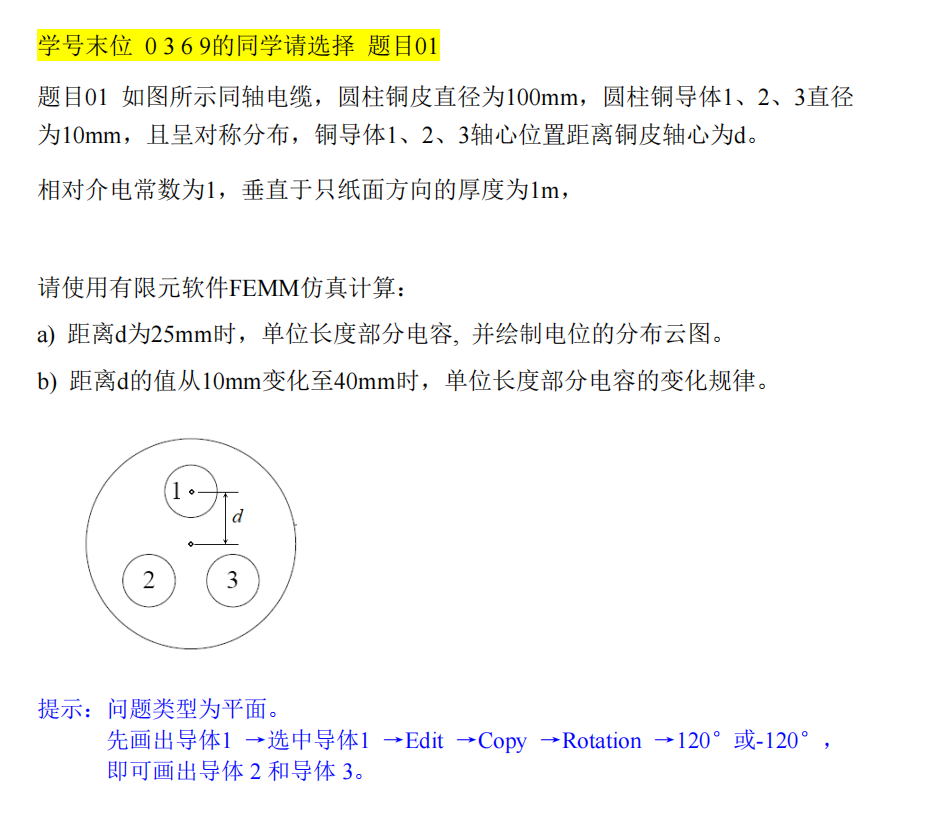
\includegraphics[width=0.6\textwidth]{题目.png}
\end{center}

\section{实验结果(a)}
内导体偏心距 \(d=25\ \text{mm}\) 时静电场电位分布云图如下：

\begin{center}
    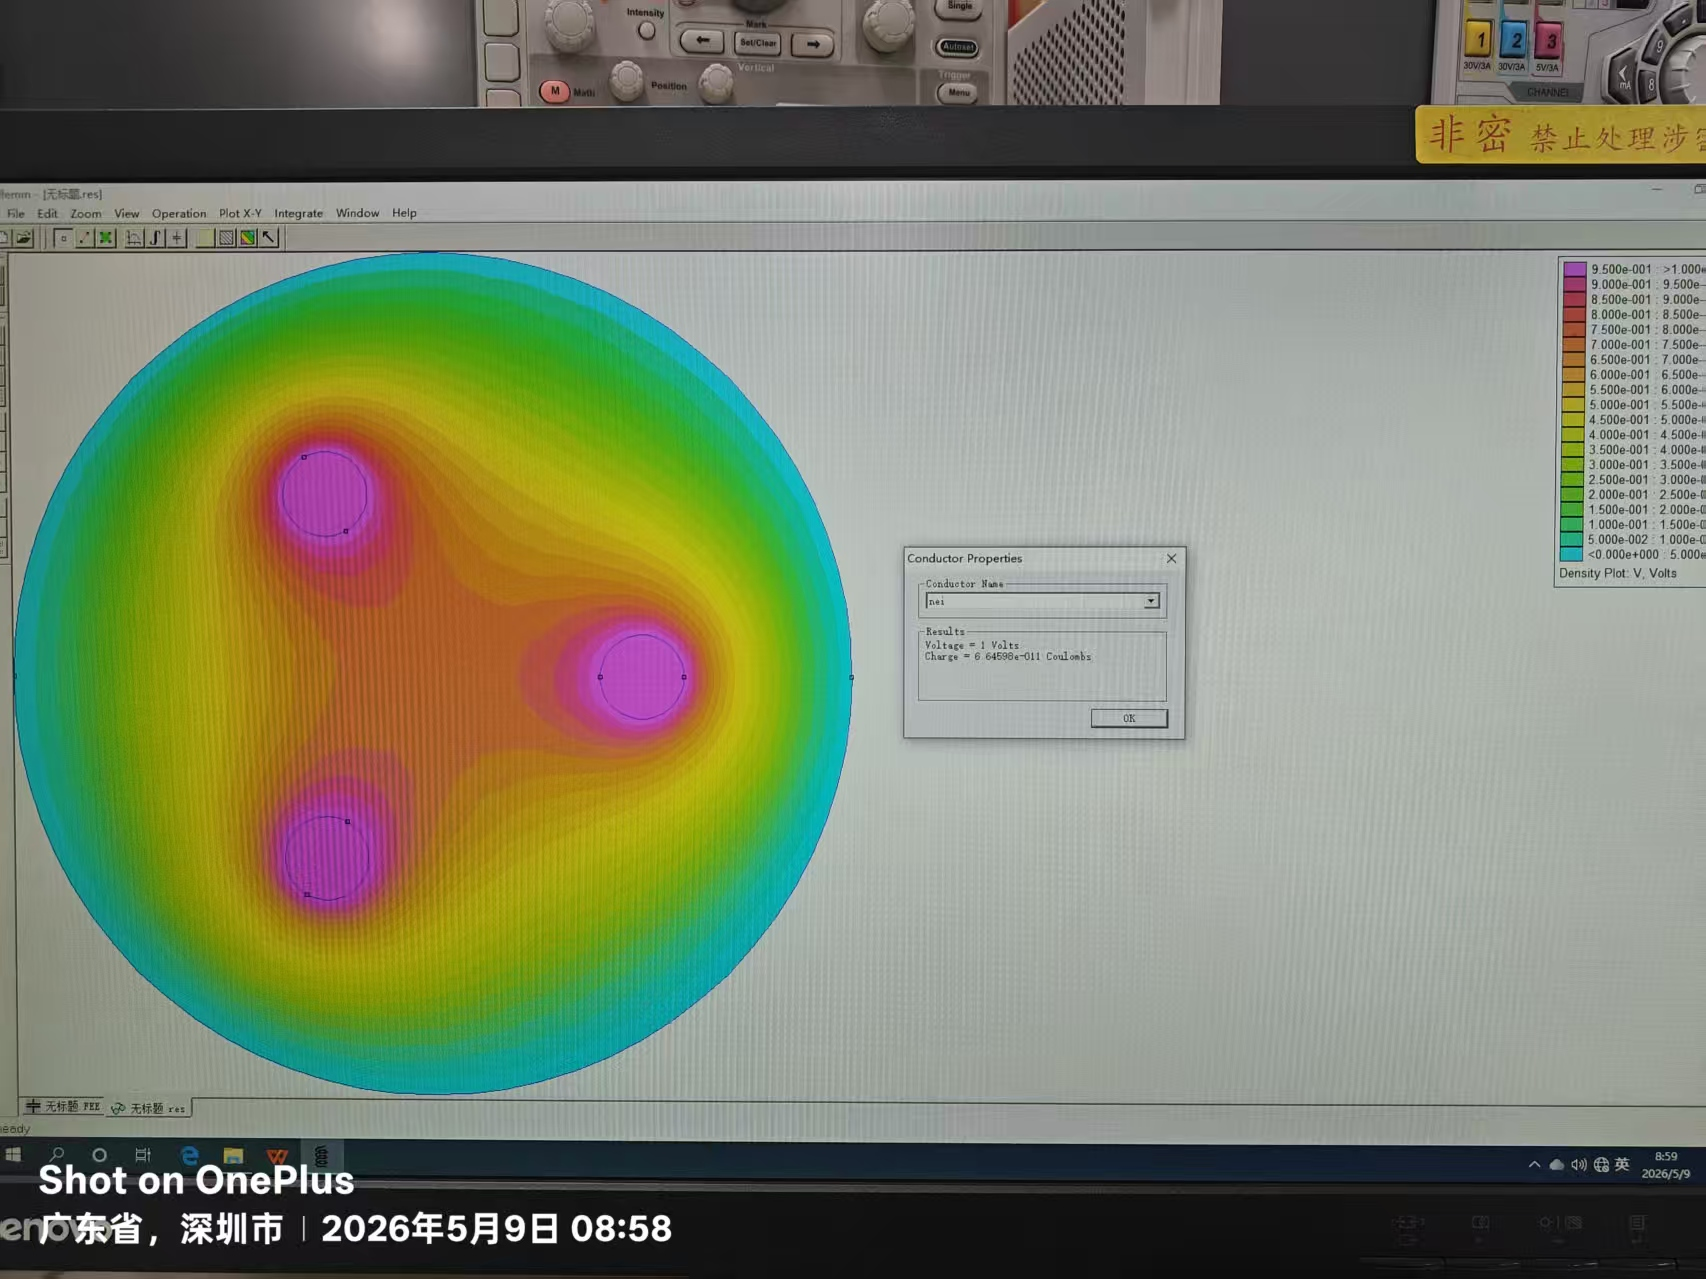
\includegraphics[width=0.8\textwidth]{1.jpg}
\end{center}
\begin{center}
    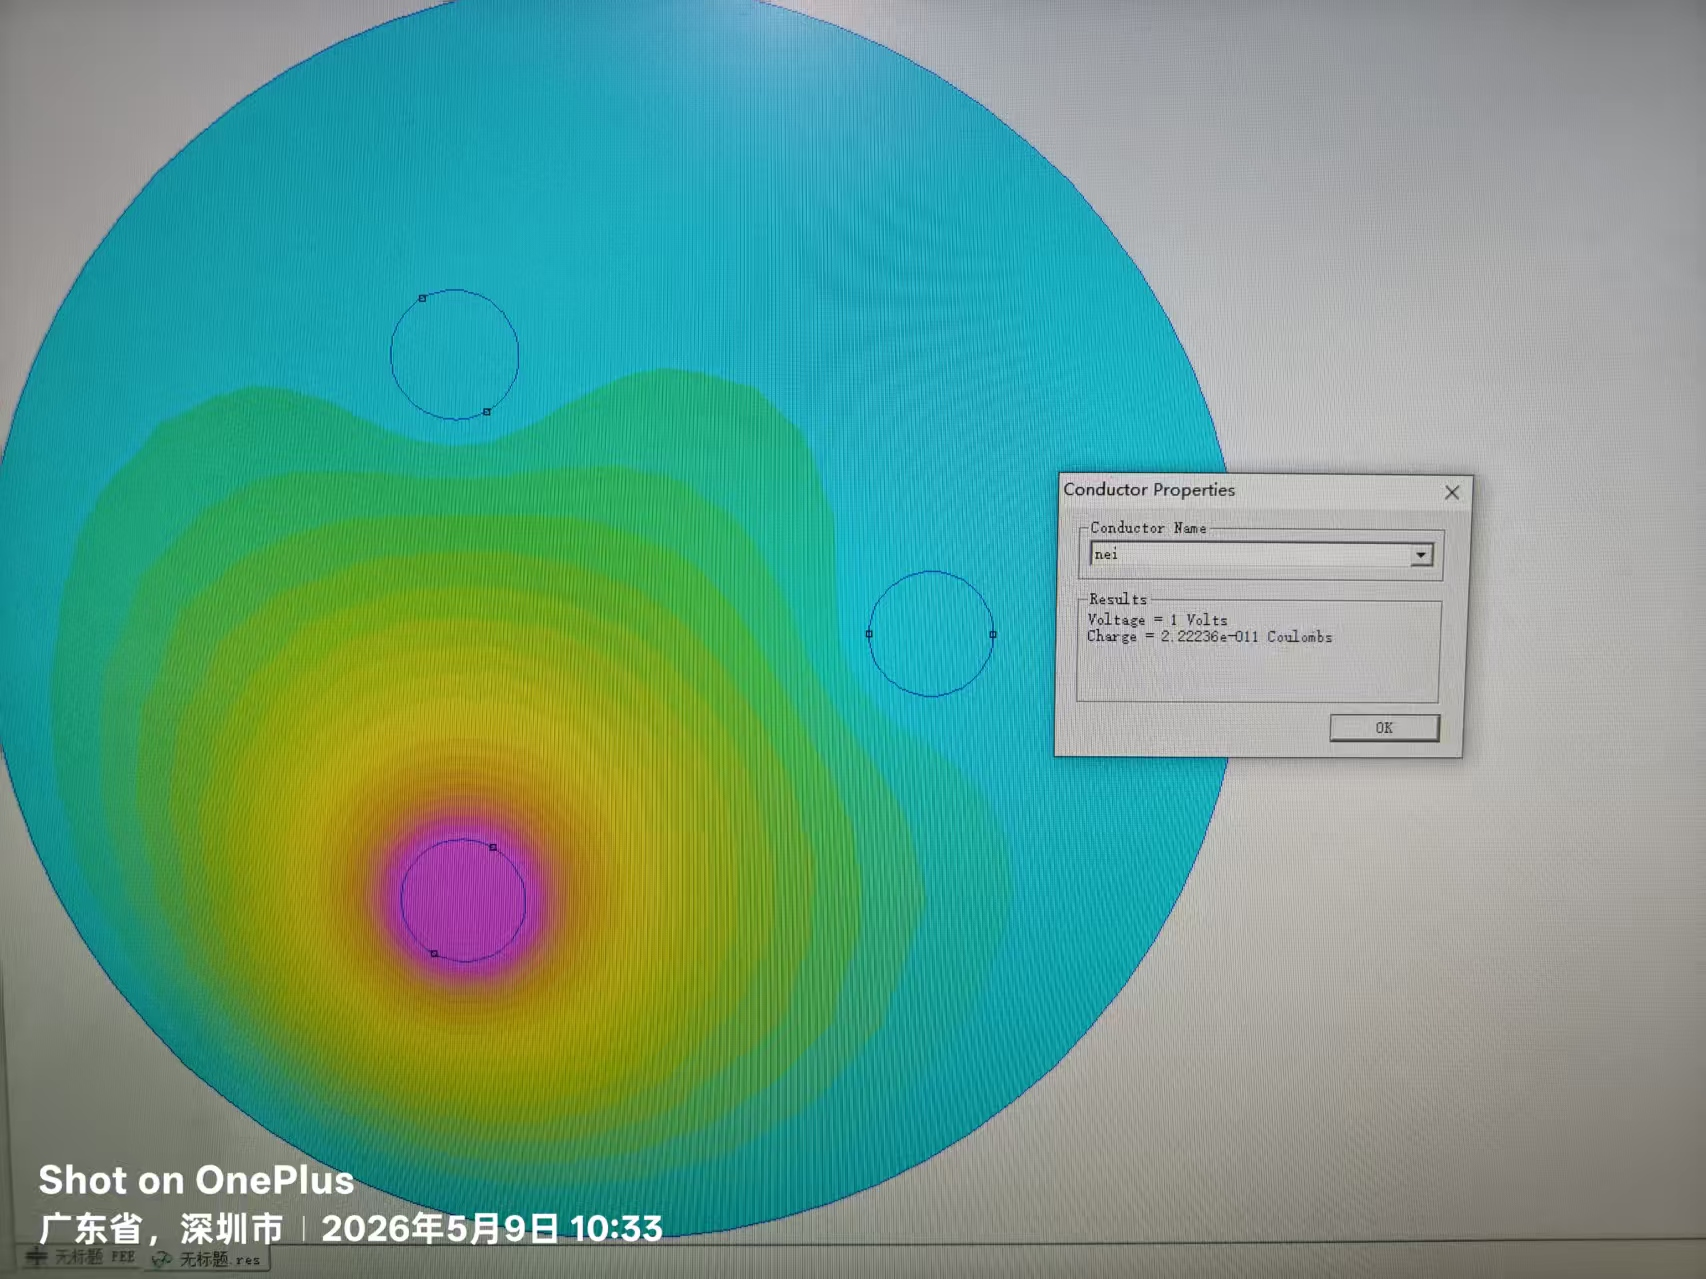
\includegraphics[width=0.8\textwidth]{2.jpg}
\end{center}

由仿真结果可见：三根内导体均为等势体，电位维持 1V；外导体边界电位为 0V，电位由内向外平滑过渡，分布规律符合静电场基本特性。

\section{实验结果(b)}
\subsection{电容数据表格}
根据 FEMM 仿真结果，计算得到不同偏心距下单位长度部分电容如下：

\begin{center}
\begin{tabular}{|c|c|}
\hline
\textbf{偏心距 \(d\) (mm)} & \textbf{单位长度部分电容 \(C\) (pF/m)} \\
\hline
10 & 1.89 \\
20 & 2.62 \\
25 & 3.94 \\
30 & 4.42 \\
40 & 7.86 \\
\hline
\end{tabular}
\end{center}

\subsection{电容变化曲线（LaTeX 直接绘制）}
\begin{center}
\begin{tikzpicture}
\begin{axis}[
    width=12cm, height=7cm,
    grid=major,
    xlabel={偏心距 \(d\) (mm)},
    ylabel={单位长度电容 \(C\) (pF/m)},
    title={同轴电缆内导体偏心距与单位长度电容关系曲线},
    xmin=0, xmax=45,
    ymin=0, ymax=8.5,
    legend pos=north west,
    mark options={solid},
]
\addplot[blue, thick, mark=circle, mark size=3pt] coordinates {
    (10, 1.89)
    (20, 2.62)
    (25, 3.94)
    (30, 4.42)
    (40, 7.86)
};
\legend{单位长度电容};
\end{axis}
\end{tikzpicture}
\end{center}

\subsection{变化规律说明}
随着内导体偏心距 \(d\) 增大，单位长度部分电容呈\textbf{单调上升趋势}，且在 \(d>30\ \text{mm}\) 后上升速率明显加快。

物理机理：内导体越靠近外导体，局部电场越集中，等效间距减小，电容显著增大；内导体越靠近中心位置，电场分布越均匀，电容越小。曲线变化趋势与静电场理论完全一致。

\end{document}